% !Mode:: "TeX:UTF-8"                                  %  采用UTF-8编码
\documentclass[a4paper,12pt]{ctexart}
\usepackage[text={150mm,240mm},left=20mm,vmarginratio=1:1]{geometry}
\usepackage{hologo}
\newcommand{\BibTeX}{\hologo{BibTeX}}
\usepackage{minted}
\usepackage{cprotect}
\usepackage{marginnote}
\usepackage{graphicx}
\graphicspath{{./figures/}}
\usepackage{natbib}
\usepackage[pdfstartview=FitH,
            CJKbookmarks=true,
            bookmarksnumbered=true,
            bookmarksopen=true,
            colorlinks=true, %注释掉此项则交叉引用为彩色边框(将colorlinks和pdfborder 同时注释掉)
            pdfborder=001,   %注释掉此项则交叉引用为彩色边框
            citecolor=blue,% magenta, cyan 文献引用的颜色设定
            urlcolor=blue,
            linkcolor=blue,
            linktocpage=true,
            pdfauthor={Marlin, China Jiliang University, <yjccjlu@gmail.com>}
           ]{hyperref}

\newcommand{\secref}[1]{第\ref{#1}节}
\newcommand{\rmk}{{\textbf{注:}}}
\newcommand{\cau}{{\textbf{警告:}}}
\newcommand{\mt}[1]{\mintinline{tex}|#1|}
\newcounter{mycnt}
\setcounter{mycnt}{1}

\title{用于处理多文档项目的文档类和宏包\thanks{本文档适用于subfiles宏包(2012/05/23)版.}}
\author{Federico Garcia
	 \\ \normalsize 翻译: \href{mailto:yjccjlu@gmail.com}{Marlin}
}
%\date{}{2015 年 2 月 14 日}

\begin{document}
\maketitle
\begin{abstract}
  使用 subfiles 宏包,编辑由一个主文档若干个子文档构成的多文档项目时会更方便。
  用户可以正常编译使用 \mt{\input} 导入子文档的主文档,也可以直接编译子文档本身,
  此时子文档使用跟主文档相同的导言区而成为完整的一份\TeX{}文档。
\end{abstract}
%\newpage
%\tableofcontents
%\newpage

\section{简介}
\LaTeX{}的 \mintinline{tex}|\include| 和 \mintinline{tex}|\input| 命令可以将多个特定的子文档编辑成一个文档。
这有利于编辑包含很多章节的大文档,但有时候在别的场合出于某种需要作者也会想要使用这样的便利。
我经常用来处理需要大量反复试错的情况,诸如较长代码的例子,表格,插图等等
\footnote{对我来说,常常需要处理的是 MusiX\TeX{} 音乐文档,代码往往很长,很复杂,而且可读性差。}。

在这种情况下,文档的其余部分很少用到,有时候甚至是一种干扰
\footnote{比如说,报错信息标识了错误的行号,甚至是错误的文档。}。
很多时候,作者只好选择新建一个文档来编辑,这意味着需要如下三个步骤:
\begin{itemize}
	\item 新建一个文档,复制粘贴主文档的导言区;
	\item 在这个例子文档中,在必要的情况下,将它单独编辑编译很多次;
	\item 得到满意的编译结果后,删掉这个新文档的导言区(包括\mintinline{tex}|\end{document}|!)然后在主文档里使用\mintinline{tex}|\include|(很多时候用的是\mintinline{tex}|\input|)导入子文档。
\end{itemize}

理想的方式是将上述三个步骤约简为值得关注的一个:中间那一步。
这就意味着每一个新建的子文档既是某个项目的一部分,也是一份完整自洽的 \LaTeX{} 文档,取决于使用 \mt{\include/ \input} 导入还是由 \LaTeX{} 编译。
这就是这份 subfiles 文档类和宏包打算做的工作。

这里主要的想法是重定义 \mt{\documentclass} 指令和 \mt{document} 环境。
在 \LaTeX{} 里这两个概念是很重要的,轻易不应改动。
就我所知,subfiles 文档类和宏包对它们作了无害的改动,而且在实现需要的功能后又小心地恢复了所作的改动。
这是 subfiles 的第一版,尽管我做了很多次的努力,它还是容易与别的文档类和宏包有冲突影响。

\section{用法}
\subsection{设置}
涉及到的文档有如下基本的结构:

\centerline{
	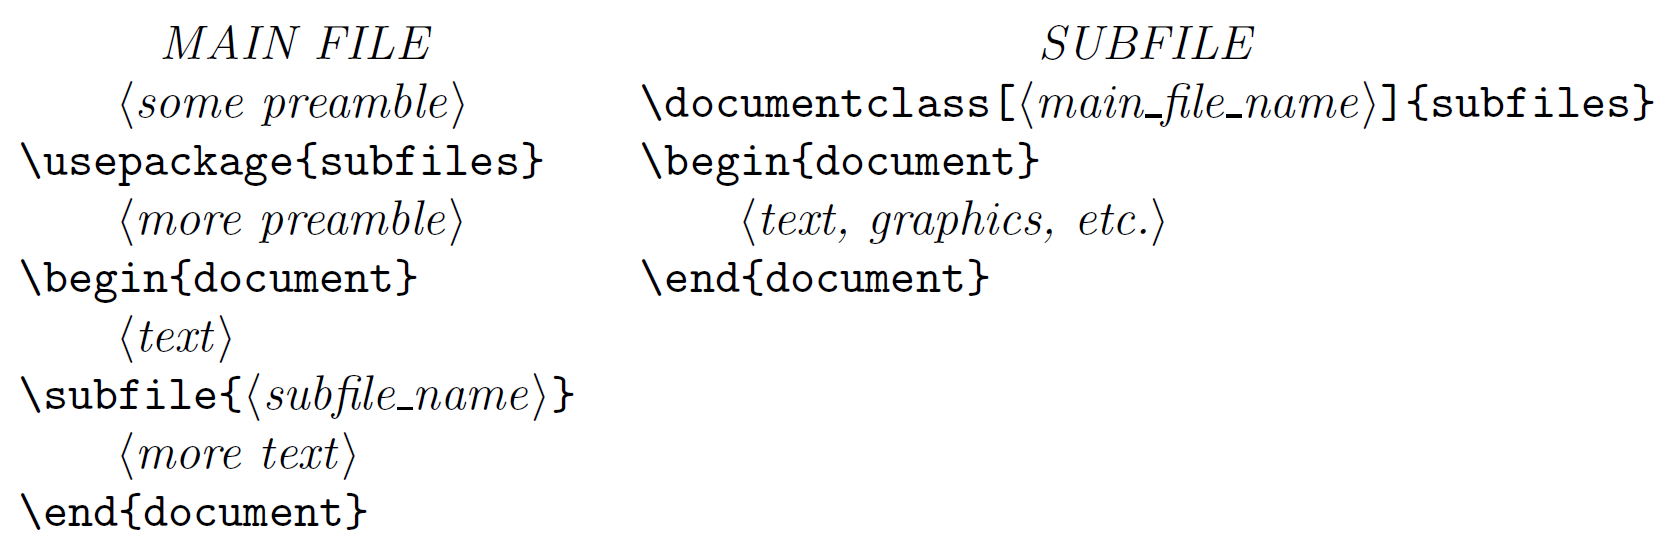
\includegraphics[width=.85\textwidth]{pic1}
}

subfiles 宏包由 \LaTeX{} 项目主文档调用,subfiles 文档类由每个子文档调用。
需要注意的是 subfiles 文档类带有一个可选项(实际上是必需的):主文档名。
这个主文档名应该带上 \TeX{} 文档默认后缀\mt{.tex},如果主文档和子文档在不同文件夹下,还需要给出主文档路径(分隔符是 \mt{/} 而不是 \mt{\ }),路径中的空格会被忽略(至少在 Windows 下)。

\subsection{结果}
这样一来,\LaTeX{} 编译主文档或子文档时会得到如下结果:
\begin{itemize}
	\item 如果排版的是子文档自身,复制主文档的导言区 ( 包括  \mt{\documentclass}),然后正常排版。
	\item 如果子文档是由\mt{\subfile}指令导入的,忽略子文档中\mt{\begin{document}}指令及其之前的所有内容,也忽略\mt{\end{document}}指令。(子文档的正文部分,实际上是被\mt{\input}到主文档的。)
\end{itemize}

\mt{\subfile}指令更像是\mt{\input}而不是\mt{\include},并不会开始新的一页。
这条指令允许嵌套,但是没有类似于\mt{\includeonly}的抑制机制。

\subsection{进一步的细节和警告}
实际上,排版子文档本身时并不只是复制主文档的导言区,而是复制了主文档在\mt{\begin{document}}和\mt{\end{document}}之外的所有内容。
这会有两个后果:
a)排版子文档本身时用户可以只读取处理到主文档导言区的那些命令;
b)用户必须很小心处理主文档中\mt{\end{document}}之后的那些内容,任何语法错误都会毁掉子文档的编译排版。

主文档的导言区可以使用\mt{\input}(注意不是\mt{\include},也不是\mt{\subfile})指令导入其他文档(例如包含定义和快捷命令的文档等),子文档的导言区也可以。
但是必须意识到每个子文档是作为一个组\mt{\input}导入的,因此在子文档里设置的定义等在子文档之外无效。
无论是否使用 subfiles, 一个好的经验是任何定义都放在主文档的导言区,避免混淆,也易于使用。

原则上,\mt{\subfile}指令可以嵌套使用,在我的测试中也确实可以正常工作,只要每一个子文档在调用subfiles文档类时使用主文档名作为选项即可。
然而我们知道在一些奇怪的情况下会有不可预期的结果。
任何情况下,subfiles都不会取代\mt{\include}和\mt{\input},它们任然有效,可以正常使用。

subfiles文档类和宏包需要调用verbatim宏包,该宏包的comment环境用来忽略不同文档的不同部分。
这不会是一个问题,因为这个宏包是包含在\LaTeXe{}标准版中的。

\section{实现}
\subsection{文档类}
\begin{minted}[xleftmargin=1cm]{tex}
1 <*class>
2 \NeedsTeXFormat{LaTeX2e}
3 \ProvidesClass{subfiles}[2012/05/23 Federico Garcia]
4 \RequirePackage{verbatim}
5 \DeclareOption*{\typeout{Preamble taken from file `\CurrentOption'}%
6     \let\preamble@file\CurrentOption}
7 \ProcessOptions
\end{minted}

首先要做的是保存常规的\LaTeX{}中的 \mt{\document},\mt{\enddocument} ,\mt{\documentclass} 等定义:
\begin{minted}[xleftmargin=1cm]{tex}
8 \let\old@document@subfiles\document
9 \let\old@enddocument@subfiles\enddocument
10 \let\old@documentclass@subfiles\documentclass
\end{minted}

现在 document 环境已经重定义为 comment。
结果就是主文档的正文部分被 \LaTeX{} 忽略,只有导言区被读出来。
(还有主文档中 \mt{\end{document}} 指令之后的任何内容!)
对子文档已经导入的 \mt{\documentclass} 指令,重定义为 \mt{\LoadClass}。
主文档的文档类和选项如是导入子文档。
\begin{minted}[xleftmargin=1cm]{tex}
11 \let\document\comment
12 \let\enddocument\endcomment
13 \let\documentclass\LoadClass\relax
\end{minted}

现在可以由 \mt{\input} 导入主文档,然后恢复原来的 \mt{\document}, \mt{\enddocument}, \mt{\documentclass} 等指令的定义。
备份命令被 \mt{\undefined} 释放以节省内存。
就好了。
\begin{minted}[xleftmargin=1cm]{tex}
14 \input{\preamble@file}
\end{minted}

这里有些不太明显的东西。
通常情况下,\verb|\preamble@file| 包含一些 \mt{\usepackage} 指令,最后使得 \verb|@| 不再是一个字符。
鉴于此,接下来需要 \mt{\catcode}命令,分组和 \verb|\global's|。
\begin{minted}[xleftmargin=1cm]{tex}
15 {\catcode`\@=11
16 \global\let\document\old@document@subfiles
17 \global\let\enddocument\old@enddocument@subfiles
18 \global\let\documentclass\old@documentclass@subfiles
19 \global\let\old@document@subfiles\undefined
20 \global\let\old@enddocument@subfiles\undefined
21 \global\let\old@documentclass@subfiles\undefined}
22 </class>
\end{minted}

\subsection{宏包}
任何选项都会被忽略。
\begin{minted}[xleftmargin=1cm]{tex}
23 <*package>
24 \NeedsTeXFormat{LaTeX2e}
25 \ProvidesPackage{subfiles}[2012/05/23 Federico Garcia]
26 \DeclareOption*{\PackageWarning{\CurrentOption ignored}}
27 \ProcessOptions
28 \RequirePackage{verbatim}
\end{minted}

宏包的核心。原理是重定义 document 环境,使得子文档的 \mt{\begin} 和 \mt{\end{document}} 容易被导入。
\mt{\documentclass} 的重定义是类似的,只是有一个要求和一个对 \mt{\subfile} 指令没有意义的可选参数。
\cprotect\marginnote{\verb|\skip@preamble|}
\begin{minted}[xleftmargin=1cm]{tex}
29 \newcommand{\skip@preamble}{%
30    \let\document\relax\let\enddocument\relax%
31    \newenvironment{document}{}{}%
32    \renewcommand{\documentclass}[2][subfiles]{}}
\end{minted}


注意新的指令 \mt{\subfile} 需要 \mt{skip@preamble} 在一个组。
在子文档被导入后,对 document 和 \mt{\documentclass} 的改动需要恢复。
\cprotect\marginnote{\verb|\subfile|}
\begin{minted}[xleftmargin=1cm]{tex}
33 \newcommand\subfile[1]{\begingroup\skip@preamble\input{#1}\endgroup}
34 </package>
\end{minted}

\end{document}